\documentclass[conference]{IEEEtran}
\IEEEoverridecommandlockouts
\usepackage{cite}
\usepackage{amsmath,amssymb,amsfonts}
\usepackage{graphicx}
\usepackage{textcomp}
\usepackage{xcolor}
\usepackage{booktabs}
\usepackage{tikz}
\usetikzlibrary{positioning,arrows.meta,fit}
\graphicspath{{figures/}}

\begin{document}

\title{LegalGPT: Measured, Cited and Verifiable Question Answering for Indian Criminal Law}

% Students: PES2UG23AM903, PES2UG23CS152, PES2UG23CS459, PES2UG23CS484. Project guide: Prof. Udayabhaskara N.
% Add an email line to each block (before the closing brace) if the venue asks for one.
\author{\IEEEauthorblockN{S Bhavish}
\IEEEauthorblockA{\textit{Dept. of CSE (AI and ML)} \\
\textit{PES University}\\
Bengaluru, India}
\and
\IEEEauthorblockN{Chinmayi Shravani}
\IEEEauthorblockA{\textit{Dept. of Computer Science and Engineering} \\
\textit{PES University}\\
Bengaluru, India}
\and
\IEEEauthorblockN{Raghav Sharma}
\IEEEauthorblockA{\textit{Dept. of Computer Science and Engineering} \\
\textit{PES University}\\
Bengaluru, India}
\and
\IEEEauthorblockN{Rithvik Hemanth}
\IEEEauthorblockA{\textit{Dept. of Computer Science and Engineering} \\
\textit{PES University}\\
Bengaluru, India}
\and
\IEEEauthorblockN{Udayabhaskara N}
\IEEEauthorblockA{\textit{Dept. of Computer Science and Engineering} \\
\textit{PES University}\\
Bengaluru, India}
}

\maketitle

\begin{abstract}
Large language models answer legal questions fluently but often cite the wrong statute, state
punishments the law does not prescribe, and treat civil disputes as crimes. We present LegalGPT, a
research system for Indian criminal law whose reliability claims are measured rather than asserted.
Answers are written only from retrieved statute text, either the Indian Penal Code or the Bharatiya
Nyaya Sanhita that replaced it in July 2024, and every claim is cited. Retrieval combines dense
search with a lay-term lexicon, a crime-scope classifier and a model-written query rewrite. Real
Supreme Court judgments, segmented into rhetorical roles by an InLegalBERT ensemble, are cited next
to the statute. A Prolog rule engine checks offence elements, a case-analysis module structures case
files without ever stating a verdict, and answers are signed, with zero-knowledge proofs of
retrieval. Paired against the same three models answering alone, LegalGPT eliminates wrong
punishments and civil questions treated as offences, which the models alone produced in up to 54 and
90 percent of cases, and raises statute-section accuracy from 41 to 81 percent to 98 to 100 percent.
The sentence-role ensemble reaches a macro-F1 of 0.807. We further evaluate Hindi questions, answering
under the new code, prompt injection, citation faithfulness with independent model judges and a blind
human check. Beyond citations, the system explains each decision: a reasoning trace whose key facts
are tested by removing them, word- and source-level perturbation, a counterfactual
bias check (gender, religion, caste, income, region, age) that separates differences the law requires
from unexplained ones, and an analysis of what
LoRA fine-tuning changed inside the local model. We release a one-command reproduction of every result.
\end{abstract}

\begin{IEEEkeywords}
legal question answering, retrieval-augmented generation, Indian Penal Code, Bharatiya Nyaya Sanhita,
rhetorical role labelling, neuro-symbolic verification, citation faithfulness, explainability,
counterfactual fairness
\end{IEEEkeywords}

\section{Introduction}

Legal questions are a high-stakes use of large language models (LLMs). A citizen describing an
incident wants to know which offence applies and what the law prescribes; a wrong section or an
invented punishment is worse than no answer. Studies of commercial legal research assistants and of
general-purpose LLMs report frequent hallucinated or misattributed authority even in
retrieval-augmented systems \cite{magesh2025hallucination,dahl2024fictions}. Indian criminal law adds
two difficulties. First, the Indian Penal Code, 1860 (IPC) \cite{ipc} was replaced by the Bharatiya
Nyaya Sanhita, 2023 (BNS) \cite{bns} for offences committed from 1 July 2024, while the IPC continues
to govern earlier offences and the existing case law; section numbers changed throughout. Second,
many users ask in Hindi, while legal text and most retrieval models are English.

Retrieval-augmented generation (RAG) \cite{lewis2020rag} grounds answers in sources, but grounding
alone does not establish that an answer is right, that its citations support it, or that the system
declines what it does not cover. We argue that a legal assistant should make each of these properties
measurable and, where possible, checkable by a third party.

This paper presents LegalGPT and makes the following contributions:
\begin{itemize}
\item A retrieval pipeline for everyday descriptions of events (a lay-term lexicon, a crime-scope
classifier and a gated LLM query rewrite) that lifts retrieval of an acceptable section on held-out
scenarios from 2 to 95 percent while answering none of 30 out-of-scope questions (Section~\ref{sec:system}).
\item Paired evaluations of three LLMs alone and inside LegalGPT, with exact McNemar tests, showing
the elimination of wrong punishments and of civil questions treated as offences (Section~\ref{sec:results}).
\item Answering under both the IPC and the BNS from their official texts, with an IPC--BNS
correspondence extracted from the official table, and Hindi question answering via translation.
\item A sentence-role (rhetorical role) ensemble for Indian judgments with context and public-corpus
transfer (macro-F1 0.807), used to build a 28,055-passage judgment library cited by the system.
\item Safety and faithfulness evaluations: element checks in Prolog, a verdict guard against
prompt injection, citation faithfulness judged by two independent models, and a blind human
spot-check of those judges.
\item Explanations of the decision itself, each tested for faithfulness: an IRAC reasoning trace
checked by fact and source perturbation, word-level importance, a counterfactual bias check aware of
the offences Indian law defines by gender, and an analysis of the LoRA update (Section~\ref{sec:xai}).
\item Verifiability (signed answers and zero-knowledge proofs) and a single command that rebuilds
every reported result from cached outputs.
\end{itemize}

\section{Related Work}

\textbf{Legal hallucination and grounded generation.} Dahl et al. profile legal hallucinations of
general LLMs \cite{dahl2024fictions}; Magesh et al. find that commercial RAG legal tools still
hallucinate in a substantial share of queries \cite{magesh2025hallucination}. RAG \cite{lewis2020rag}
and citation-generating models \cite{gao2023citations} improve grounding, and Liu et al. show that
generative search engines often cite sources that do not fully support their statements
\cite{liu2023verifiability}. We measure the same failure modes on Indian criminal law and add
abstention on out-of-scope questions as a first-class metric.

\textbf{Indian legal NLP.} InLegalBERT is a BERT model pre-trained on Indian legal text
\cite{paul2023inlegalbert}. Rhetorical role labelling of Indian judgments was introduced by
Bhattacharya et al. \cite{bhattacharya2019roles}; Kalamkar et al. released the InRhetoricalRoles
corpus \cite{kalamkar2022corpus}; ILDC addresses judgment prediction \cite{malik2021ildc}. We do not
predict outcomes; we use roles to choose which passages of a judgment may be cited.

\textbf{Logic and law.} Encoding legislation as logic programs dates back to the British Nationality
Act in Prolog \cite{sergot1986bna}. We use SWI-Prolog \cite{wielemaker2012swi} for offence elements and
combine it with LLM fact extraction, each fact anchored to a quote.

\textbf{Model judges and prompt injection.} LLM-as-a-judge evaluation \cite{zheng2023judge} is common
but its agreement with people must be checked; we report agreement with a blind human annotator.
Indirect prompt injection through processed documents \cite{greshake2023injection} is directly
relevant when users upload case files.

\section{System}\label{sec:system}

Fig.~\ref{fig:arch} shows the two halves of the system: an offline pipeline that builds a
role-labelled judgment library, and the online path every question takes.

\begin{figure*}[t]
\centering
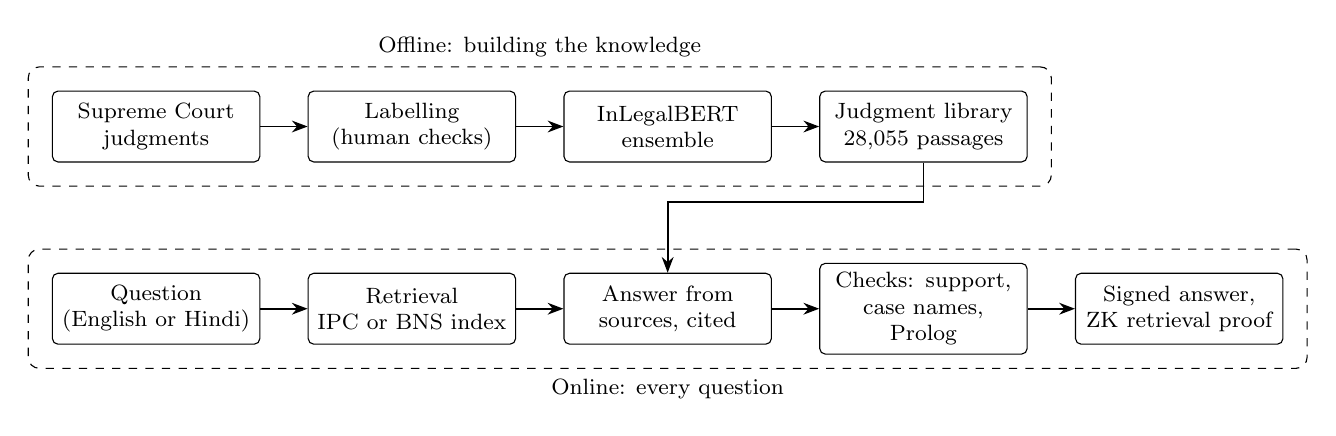
\begin{tikzpicture}[
  node distance=4mm and 6mm,
  box/.style={draw, rounded corners=2pt, align=center, font=\footnotesize, minimum height=9mm, text width=24mm, fill=white},
  lane/.style={draw, dashed, rounded corners=4pt, inner sep=3mm},
  arr/.style={-{Stealth[length=2mm]}, semithick}]
\node[box] (j) {Supreme Court\\judgments};
\node[box, right=of j] (l) {Labelling\\(human checks)};
\node[box, right=of l] (m) {InLegalBERT\\ensemble};
\node[box, right=of m] (lib) {Judgment library\\28,055 passages};
\draw[arr] (j) -- (l); \draw[arr] (l) -- (m); \draw[arr] (m) -- (lib);
\node[box, below=14mm of j] (q) {Question\\(English or Hindi)};
\node[box, right=of q] (r) {Retrieval\\IPC or BNS index};
\node[box, right=of r] (a) {Answer from\\sources, cited};
\node[box, right=of a] (c) {Checks: support,\\case names, Prolog};
\node[box, right=of c] (s) {Signed answer,\\ZK retrieval proof};
\draw[arr] (q) -- (r); \draw[arr] (r) -- (a); \draw[arr] (a) -- (c); \draw[arr] (c) -- (s);
\draw[arr] (lib.south) -- ++(0,-5mm) -| (a.north);
\node[lane, fit=(j)(lib), label={[font=\footnotesize]above:Offline: building the knowledge}] {};
\node[lane, fit=(q)(s), label={[font=\footnotesize]below:Online: every question}] {};
\end{tikzpicture}
\caption{LegalGPT. Judgments are segmented into rhetorical roles to build a citable library
(top); each question is retrieved against the IPC or BNS, answered only from the retrieved sources,
checked and signed (bottom). Case analysis runs both halves on an uploaded case file.}
\label{fig:arch}
\end{figure*}

\subsection{Corpus and retrieval}

The IPC text from India Code was parsed into a section, sub-section and clause hierarchy (all 574
sections, 685 chunks of at most 1,400 characters, each tagged with its citation path). The BNS text
(Act 45 of 2023) was parsed with the same parser into its own index (all 358 sections, 479 chunks).
Chunks are embedded with all-MiniLM-L6-v2 \cite{wang2020minilm,reimers2019sbert} and stored in a
vector database.

Embedding search alone rarely bridges everyday wording (``someone took my bicycle from my shed'')
and statutory language. Three components close the gap. A lay-term lexicon of 41 rules maps
everyday expressions to statutory terms. A logistic-regression scope classifier on the question
embedding estimates whether the question concerns a crime; it lowers the similarity floor for crime
questions and is trained on 486 practice questions (never the held-out ones), with its threshold set
above every out-of-scope validation question. Finally, an LLM rewrite names the likely offences and
sections; the rewrite only steers retrieval (the named sections' text is fetched) and is used only
when the scope classifier agrees that the question concerns a crime, so civil questions are still
declined whatever the LLM says. Definition questions additionally fetch the section titled with the
defined term.

\subsection{Answering and citation rules}

The answering model receives the numbered sources and a fixed set of rules: answer only from the
sources, cite every claim with its source number, quote punishments exactly, apply defined offences
to described facts, and reply with a fixed refusal when no source covers the question. Answers are
produced by hosted models on free tiers (gpt-oss-120b \cite{openai2025gptoss} by default, and Gemini)
or by local Qwen2.5 models \cite{qwen2024qwen25} fine-tuned with LoRA \cite{hu2022lora} and quantized
\cite{dettmers2023qlora} for fully offline use.

\subsection{IPC and BNS}

An IPC--BNS correspondence was extracted from the official table of the Bureau of Police Research and
Development \cite{bprd2024table}, rebuilt from the PDF's text positions; it maps 527 IPC sections,
lists 23 BNS provisions with no IPC source, and agrees with all 47 entries of an earlier unverified
map. Questions are answered under the BNS when the user selects it, names it, or dates the events on
or after 1 July 2024, and under the IPC otherwise. Under the BNS, the rewrite's IPC sections are
converted to BNS sections through the table before retrieval, and every source shows the IPC
section(s) it replaced; IPC answers show the BNS equivalent of each cited section. The numbers shown
come from the table, never from the model.

\subsection{Hindi}

A question written mostly in Devanagari is translated to English by the answering model (or another
free hosted model) for retrieval, and the answer is requested in Hindi with the same section numbers
and citations. If no model can translate, the system says so instead of declining for lack of a
match.

\subsection{Sentence roles and the judgment library}

Each sentence of a judgment is labelled Facts, Law Applied, Precedent, Argument or Ruling. The
classifier fine-tunes InLegalBERT \cite{paul2023inlegalbert} on the sentence with its position and
neighbouring sentences, and averages its probabilities with a BiLSTM \cite{hochreiter1997lstm} that
reads the whole judgment over frozen sentence vectors. Both members were pre-trained on the
InRhetoricalRoles corpus \cite{kalamkar2022corpus} (its 13 roles mapped onto our five). In the
labelling interface the model's suggestions are checked by people; sentences below a confidence of
0.9, and a random sample above it, are reviewed, and about one judgment in ten is labelled blind with
suggestions hidden, to keep measuring the model.

The library holds 349 judgments: 312 Supreme Court criminal judgments from 2020--2023 that cite the
IPC (from a public CC-BY-4.0 collection \cite{scjudgments}), labelled by the ensemble, and our 37
annotated judgments, a total of 28,055 role-labelled passages. The chat cites at most two Ruling, Law
Applied or Precedent passages (one per judgment, similarity at least 0.60), only when statute
retrieval succeeded.

\subsection{Explanation and checks}

Every answer carries an explanation: the evidence match between the question and the retrieved law,
the source supporting each sentence (embedding similarity), and warnings for citations outside the
sources or sentences that cite one judgment while naming another. Seven IPC sections (279, 304A,
304B, 323, 337, 338, 379) are encoded as element checklists in Prolog \cite{wielemaker2012swi}. An
LLM extracts the facts each element depends on, each with a quote from the user's text that must
appear verbatim, and the engine returns consistent, inconsistent or insufficient, naming the facts
that would change the verdict.

\subsection{Explaining the decision}\label{sec:xai}

Citations show where an answer came from, not why the model concluded it. LegalGPT therefore explains
the decision itself, and tests every explanation, since post-hoc explanations can be unfaithful
\cite{turpin2023unfaithful,jacovi2020faithfulness}. Hosted models are black boxes, so their decisions
are explained by perturbation: the input is changed and the output observed. Our own fine-tuned model
is open, so it is also explained from its weights.

\textbf{Reasoning trace.} After an answer, the model sets out its reasoning in the IRAC form used in
legal writing: the issue, each retrieved section with whether and why it applies, each fact matched to
an element, and the conclusion with the facts it depends on (key facts, quoted from the question). The
server removes any section or source number not among the sources.

\textbf{Perturbation tests.} \emph{Fact influence}: each key fact, and each other clause of the
question, is removed in turn and the answer is written again from the same sources; a fact the model
relied on changes the sections the answer relies on. The agreement between ``named as key'' and
``changes the conclusion'' is the trace's faithfulness. \emph{Source influence}: each section is left
out in turn; a section is decisive if the conclusion changes. \emph{Key words}: each word of the
question is removed and the similarity to each retrieved section and the scope classifier's crime
probability are recomputed, without any model call, giving a word-level heat map. Every model-based
test first answers the unchanged input again; changes this control also shows are run-to-run variation
and are not counted.

\textbf{Bias check.} A counterfactual fairness test \cite{kusner2017counterfactual}: the question or
case file is rewritten with only the people's gender swapped (husband and wife, pronouns, names), or
their religion (names, places), caste, income level, region or age, and both versions run through the
same pipeline together with a control run. When the text names none of the last four, one sentence
about the accused is added to two otherwise identical copies. Indian criminal law is itself gender-specific in places: dowry death (IPC 304B) is the
death of a woman, cruelty under 498A is by a husband or his relatives, rape under 375 is by a man. A
curated list of 27 such IPC offences, mapped to the BNS through the official table, separates
differences the law requires from unexplained ones; when a gender-specific offence stops applying,
the general offences that replace it (hurt, culpable homicide) are attributed to it too. Sections an
answer names only to rule them out are not counted, and stereotyped or victim-blaming wording is
flagged. The check runs automatically when a question or case file is gender-sensitive.

\textbf{Inside the local model.} Following the analysis of low-rank updates in the LoRA paper
\cite{hu2022lora}, the adapter's update $\Delta W = BA$ is examined per layer and module: its size
relative to the base weight, its effective rank, and the amplification factor
$\lVert\Delta W\rVert_F / \lVert U^\top W V\rVert_F$. Running locally, the tuned model's answer is also
scored token by token under the tuned and the base weights, and with each source removed from the
prompt, which measures inside the model which sources the answer depends on.

\subsection{Case analysis}

For an uploaded case file, the system extracts facts with verified quotes, proposes IPC offences and
validates them (the section must exist and its title must match the named offence), checks elements
(Prolog where encoded, the model otherwise), retrieves similar judgments through their Facts
passages, and writes a cited analysis. It never states or predicts a verdict. The file is fenced and
declared untrusted, fact candidates that read as instructions are dropped, and an output guard
removes sentences that state a verdict, cite a non-existent section, name a case outside the sources
or repeat the system prompt. The guard combines patterns with a logistic-regression verdict
classifier on sentence embeddings. A file with no IPC offence (for example a bail application under a
special statute) is explained as out of scope rather than analysed.

\subsection{Verifiability}

Every answer is signed with Ed25519 \cite{bernstein2012ed25519} over the question, prompt, cited
sources and answer. Using EZKL \cite{ezkl}, a zero-knowledge proof shows that a verdict follows from
the published rules for the extracted facts without revealing them, and that an answer's IPC sources
are exactly those the retrieval rules select from all 685 chunks.

\section{Evaluation Setup}

\textbf{Benchmark.} The benchmark has 365 statute questions generated from the IPC (punishment and
definition), 308 everyday scenarios with acceptable sections, and 54 out-of-scope (civil or general)
questions. A fixed held-out sample (seed 7) of 40 punishment, 20 definition, 60 scenario and 30
out-of-scope questions is scored once; all design decisions used other questions. Two statute
questions are malformed and excluded, so statute $n=59$ and punishment $n=39$. Scenario and
out-of-scope labels were written with AI assistance (silver labels).

\textbf{Systems and metrics.} Three hosted models (gpt-5.4-mini, Gemini 3.5 flash-lite, gpt-oss-120b)
are each evaluated alone (closed book) and inside LegalGPT on the same questions. Metrics: right
section (statute questions), acceptable section cited (scenarios), wrong punishment (a term the
section does not mention), and civil question answered as an offence. Comparisons are paired, with
exact McNemar tests \cite{mcnemar1947}; classifier comparisons add 95 percent confidence intervals
from a bootstrap \cite{efron1993bootstrap} that resamples whole judgments. Agreement uses Cohen's
kappa \cite{cohen1960kappa}.

\section{Results}\label{sec:results}

\subsection{Accuracy and safety against the models alone}

Table~\ref{tab:headline} and Fig.~\ref{fig:safety} compare each model with itself inside LegalGPT.
With all three models, LegalGPT states no wrong punishment and treats no civil question as an
offence; the models alone did both often ($p \le 0.031$). Statute-section accuracy rises to 98--100
percent ($p \le 0.002$). On scenarios LegalGPT is at least at parity: significantly better with
Gemini (93 vs 78 percent, $p=0.035$), ahead but not significantly with gpt-5.4-mini, and level with
gpt-oss-120b. Five percent of scenarios are declined by each model inside LegalGPT.

\begin{table}[t]
\caption{Model alone vs. inside LegalGPT (held-out set, exact McNemar $p$)}
\label{tab:headline}
\centering
\footnotesize
\setlength{\tabcolsep}{3pt}
\begin{tabular}{llrrrl}
\toprule
Model & Measure & $n$ & Alone & LegalGPT & $p$ \\
\midrule
gpt-5.4-mini & Right section & 59 & 75\% & \textbf{100\%} & $<$0.001 \\
 & Acceptable (scenario) & 60 & 83\% & 93\% & 0.18 \\
 & Wrong punishment$\downarrow$ & 39 & 15\% & \textbf{0\%} & 0.031 \\
 & Civil as offence$\downarrow$ & 30 & 47\% & \textbf{0\%} & $<$0.001 \\
\midrule
Gemini 3.5 & Right section & 59 & 81\% & \textbf{98\%} & 0.002 \\
flash-lite & Acceptable (scenario) & 60 & 78\% & \textbf{93\%} & 0.035 \\
 & Wrong punishment$\downarrow$ & 39 & 15\% & \textbf{0\%} & 0.031 \\
 & Civil as offence$\downarrow$ & 30 & 47\% & \textbf{0\%} & $<$0.001 \\
\midrule
gpt-oss-120b & Right section & 59 & 41\% & \textbf{100\%} & $<$0.001 \\
 & Acceptable (scenario) & 60 & 85\% & 82\% & 0.79 \\
 & Wrong punishment$\downarrow$ & 39 & 54\% & \textbf{0\%} & $<$0.001 \\
 & Civil as offence$\downarrow$ & 30 & 90\% & \textbf{0\%} & $<$0.001 \\
\bottomrule
\end{tabular}
\end{table}

\begin{figure}[t]
\centering
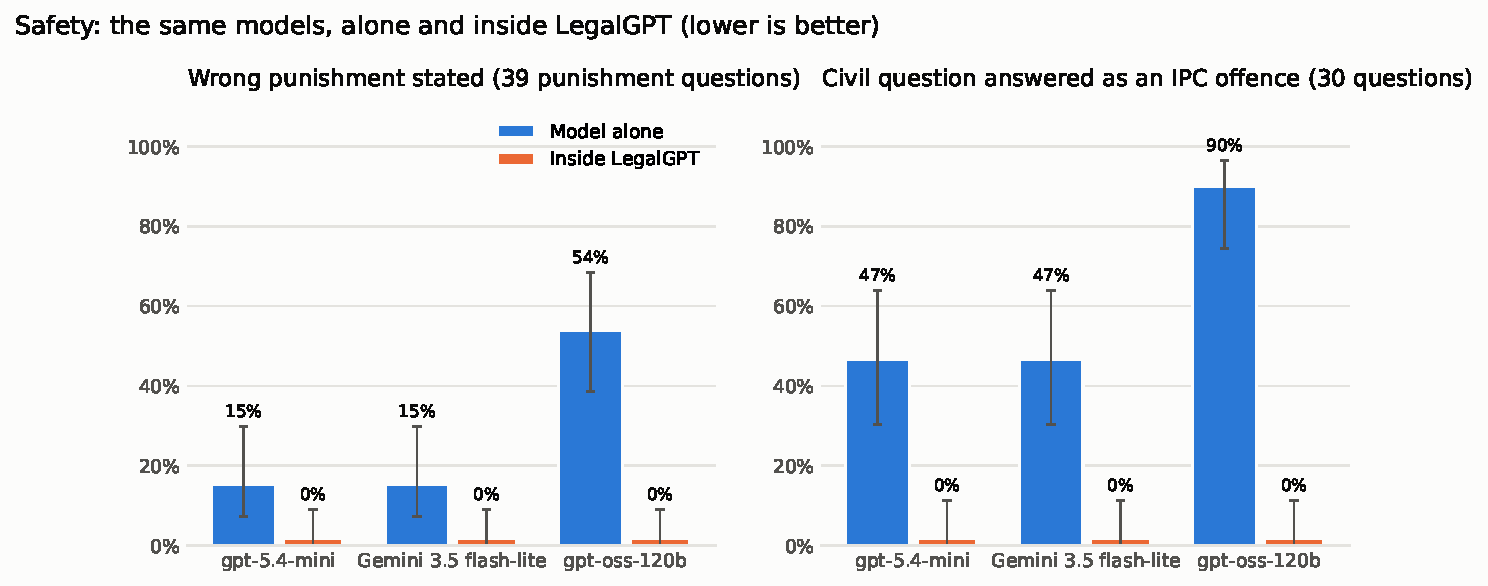
\includegraphics[width=\columnwidth]{fig1_safety.pdf}
\caption{Wrong punishments and civil questions answered as offences, the same models alone and inside
LegalGPT (lower is better).}
\label{fig:safety}
\end{figure}

\subsection{Where the gains come from}

Fig.~\ref{fig:ablation} adds retrieval components one at a time on the 60 held-out scenarios.
Embedding search alone reaches an acceptable section for 2 percent of them; the lexicon and scope
classifier lift this to 45--50 percent, the LLM rewrite to 90 percent and the retrained scope
classifier to 95 percent (88 percent with gpt-oss-120b's rewrites). No out-of-scope question is
answered at any step. End to end, the original pipeline cited an acceptable section for 43--45
percent of scenarios and the final one for 82--93 percent (each $p<0.001$; 76 questions improved,
none got worse).

\begin{figure}[t]
\centering
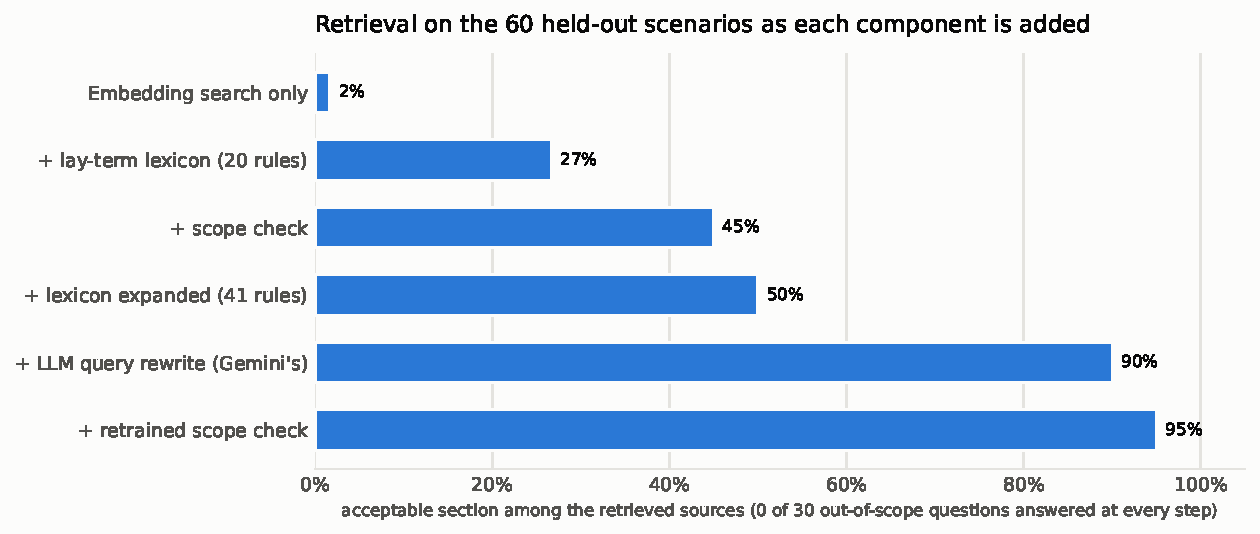
\includegraphics[width=\columnwidth]{fig3_ablation.pdf}
\caption{Retrieval on the held-out scenarios as each component is added.}
\label{fig:ablation}
\end{figure}

\subsection{Offline models}

Qwen2.5 models of 1.5B, 3B and 7B parameters, LoRA-trained on identical data and run fully offline
(each writing its own rewrite), reach 90, 100 and 98 percent statute-section accuracy and 50, 60 and
65 percent acceptable scenario sections, with no civil question treated as an offence at any size and
no wrong punishment at 3B and 7B. The gap to hosted models on scenarios comes from the local models'
own rewrites, which name an acceptable section for only 57--58 percent of scenarios; the same
pipeline reaches 82--90 percent with a large hosted model writing the rewrite.

\subsection{Sentence roles}

Under 5-fold cross-validation grouped by judgment (36 judgments, 4,823 sentences), context helps:
the sentence alone scores a macro-F1 of 0.667, position and neighbours 0.739 (Fig.~\ref{fig:rrl}).
The final ensemble, with transfer from InRhetoricalRoles, reaches 0.807 (accuracy 81.3 percent),
$+0.068$ over the deployed single model (95 percent CI $+0.041$ to $+0.096$, McNemar $p=3\times10^{-21}$).
The weakest classes gain most (Law Applied 0.632 to 0.750, Precedent 0.716 to 0.832). Of the
labelled sentences, 529 (11 percent) were labelled or confirmed by an AI assistant; scoring only the
32 judgments labelled by people gives 0.752 vs 0.813, so the gain does not depend on them. At a
confidence of at least 0.9 the ensemble covers 40 percent of sentences at 96.8 percent accuracy.

\begin{figure}[t]
\centering
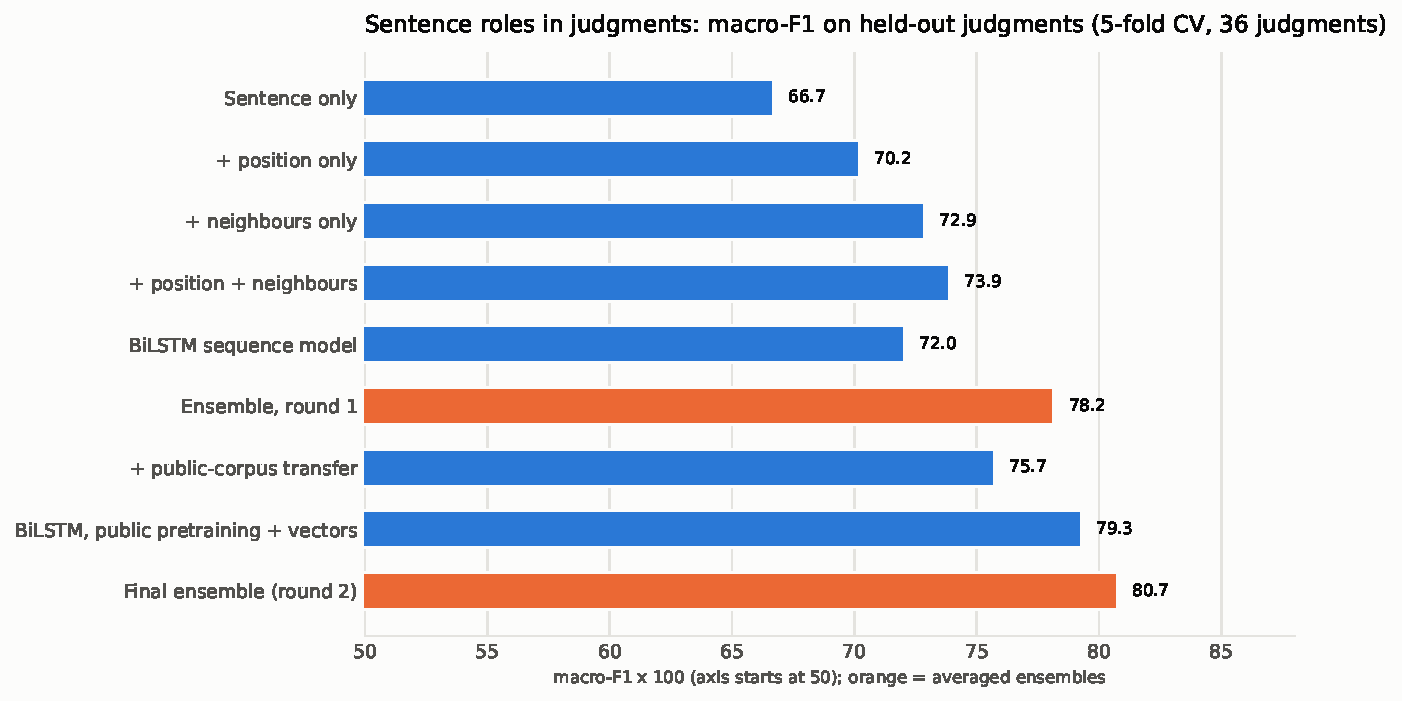
\includegraphics[width=\columnwidth]{fig5_rrl.pdf}
\caption{Sentence-role macro-F1 on held-out judgments (5-fold cross-validation).}
\label{fig:rrl}
\end{figure}

\subsection{BNS and Hindi}

With the scenarios' acceptable sections converted to BNS sections, retrieval from the BNS index finds
one for 53 of 60, the same as the IPC index (53 of 60); without the rewrite it finds 32 of 60. For
Hindi, the 90 held-out questions were machine-translated (Table~\ref{tab:bnshindi}). Searched as
written, Hindi questions retrieve nothing (0 of 60); translated first, 52 of 60. End to end with
gpt-oss-120b, 56 of 60 Hindi scenarios are answered, all in Hindi, and 51 cite an acceptable section;
all 30 out-of-scope questions are declined in Hindi. One of the 90 translations was in Urdu script;
it was found by the human check below, re-translated, and the results were unchanged.

\begin{table}[t]
\caption{BNS and Hindi: acceptable section retrieved (60 scenarios) and out-of-scope answered (30)}
\label{tab:bnshindi}
\centering
\footnotesize
\begin{tabular}{lrr}
\toprule
Condition & Retrieved & Out of scope$\downarrow$ \\
\midrule
English, IPC index & 53/60 & 0/30 \\
English, BNS index & 53/60 & 0/30 \\
English, BNS index, no rewrite & 32/60 & 0/30 \\
Hindi as written & 0/60 & 0/30 \\
Hindi, rewrite reads the Hindi & 1/60 & 0/30 \\
Hindi, translated first & \textbf{52/60} & 0/30 \\
\bottomrule
\end{tabular}
\end{table}

\subsection{Element checks and case analysis}

On 147 paired counterfactual fact patterns, adding the Prolog rules to an LLM raised accuracy from
92 to 95 percent, made every one-fact flip change the verdict correctly (95 to 100 percent), and
improved the detection of an omitted element (77 to 85 percent), at a small cost in paraphrase
consistency (100 to 95 percent); the overall difference is a trend ($p=0.23$).

Case analysis was evaluated on 120 Supreme Court judgments whose facts were given with every section
number masked; the gold offences are those cited in the judgment's own Facts and Ruling passages. The
system named at least one correct offence for 65 percent of them (95 percent CI 57--73 percent;
precision 0.45, recall 0.35), and the most similar retrieved judgment shared a gold offence in 68
percent. The IPC validation filter removed 15 proposals, five of them correct: it is a safety filter
against non-IPC section numbers rather than an accuracy gain.

\subsection{Prompt injection and the verdict guard}

Twenty-four case files carried an injected instruction (12 attacks, mid-file and at the end) aiming
at a verdict, fake law, dropped citations, a prompt leak or a code word. With Gemini 3.5 flash-lite,
1 of 24 attacks succeeded without the defences (the code word copied into offence names) and none
with them. Because the model itself resisted most attacks, we also tested the worst case: attack
sentences inserted into real analyses, as a fully compromised model would write them
(Table~\ref{tab:guard}). The verdict classifier was trained on sentences written by gpt-oss-120b and
tested on sentences written by another model family (qwen3.8-27b). It raises the share of
paraphrased verdicts caught from 18 to 93 percent without removing any of 100 sentences of real
analyses; on 125 deliberately difficult non-verdict sentences (bail, procedure, what a past court
held) it removes 13.

\begin{table}[t]
\caption{Output guard: attack sentences removed (worst case) and held-out verdicts caught}
\label{tab:guard}
\centering
\footnotesize
\begin{tabular}{lrr}
\toprule
 & Patterns & + classifier \\
\midrule
Inserted verdicts removed & 120/192 & \textbf{192/192} \\
Inserted fake law removed & 120/144 & \textbf{144/144} \\
Inserted prompt leaks removed & 72/96 & 72/96 \\
Genuine sentences removed & 0 & 0 \\
\midrule
Held-out verdicts caught & 22/120 & \textbf{112/120} \\
Real-analysis sentences removed & 0/100 & 0/100 \\
Hard non-verdicts removed & 0/125 & 13/125 \\
\bottomrule
\end{tabular}
\end{table}

\subsection{Citation faithfulness and a human check of the judges}

In 92 answers, 19 sentences cite a judgment. Two independent model judges (gpt-oss-120b and
qwen3.8-27b), each blind to the other, labelled whether the cited passage supports the sentence:
both labelled 14 of 19 supported and no sentence was labelled unsupported by both, with agreement of 0.895 and Cohen's kappa of
0.72 (0.35 on a control set of 19 statute citations). No sentence named a judgment other than the
one it cited.

Because model judges can be wrong, one author (not a lawyer) labelled all 38 citations blind to the
model labels, with the same definitions (Table~\ref{tab:spot}). The human found 31 supported, 7
partially supported and none unsupported; agreement with the judges was 76 and 79 percent (kappa
0.36), and 87 percent where both judges agreed. Every ``unsupported'' label came from a model judge,
in two cases for a sentence the cited text states verbatim, so the model-judged faithfulness is, if
anything, conservative. After comparing with a second reading, the annotator changed four labels;
we report the blind labels as the measurement.

\begin{table}[t]
\caption{Blind human labels of 38 citations vs. two model judges}
\label{tab:spot}
\centering
\footnotesize
\begin{tabular}{lrr}
\toprule
 & gpt-oss-120b & qwen3.8-27b \\
\midrule
Agreement with the human & 76\% & 79\% \\
Cohen's kappa (3-way) & 0.36 & 0.36 \\
Cohen's kappa (supported vs. not) & 0.47 & 0.42 \\
\midrule
\multicolumn{3}{l}{Human: 31 supported, 7 partial, 0 unsupported} \\
\bottomrule
\end{tabular}
\end{table}

\subsection{Explaining the decision: are the explanations faithful?}\label{sec:xai-results}

\textbf{Key words.} On 57 held-out scenarios (no model calls), removing the single word the explanation
ranks highest lowers the similarity to the top retrieved section by 0.173 on average, against 0.019 for
a random content word, and by more than a random word in every question; for the scope classifier's
crime probability the drops are 0.074 and 0.010. The deletion test follows ERASER
\cite{deyoung2020eraser}: the ranking reflects what retrieval actually uses.

\textbf{Reasoning traces.} On 18 held-out scenarios answered by Gemini 3.5 flash-lite (two others were
declined), 97 percent of the key facts named in the traces were quoted verbatim from the question, and
0.9 invalid sections or source numbers per trace were removed. Of 38 key facts, 26 (68 percent) changed
the conclusion when removed; the mean agreement between ``named as key'' and ``changes the conclusion''
was 0.70. Of the 36 sections a trace said apply, 31 were decisive when left out (precision 0.86;
recall 0.65 of the 48 decisive sections). The control run changed the result in a third to a half of
the cases, so without it a large share of ``influence'' would have been run-to-run variation. The
traces are thus largely but not fully faithful, which is why the app shows the test next to the trace.

\textbf{Bias check.} On 40 scenario pairs (24 gender-sensitive, 16 where gender should not matter), both
versions were run twice, and a section counts only if it holds in both runs of one version and neither run
of the other, with the definition and the punishment of one offence counted once. With gpt-oss-120b the
check attributed most differences in the sensitive cases to the law itself (17 pairs for the model alone,
16 inside LegalGPT). Possible bias remained in 5 of 40 pairs for the model alone and 4 inside LegalGPT, and
in 9 and 8 with Gemini 3.5 flash-lite. Neither difference is significant (exact McNemar $p=1.0$ for both),
so we do not claim that LegalGPT changes gender sensitivity. A first run with one control flagged 12 and 9,
and 20 and 13; most of those pairs did not hold when run again, which is why the stricter rule is used. A
gender-specific offence was still relied on after the genders were reversed, and so probably misapplied, in
10 pairs for the model alone and 7 inside LegalGPT, and in 17 and 15 with Gemini. No stereotyped wording was
found. The check makes the remaining cases visible to the user.

\textbf{Caste, income, region and age.} We also ran 10 scenarios per attribute where none of these
should matter. The two versions differ in one sentence about the accused (an upper-caste or a Dalit
family; a wealthy businessman or a poor daily-wage labourer; a local resident or a migrant worker from
Bihar; aged 30 or 70), except in 3 age scenarios, where an age word in the text is swapped instead. As for gender, both versions run twice and a section counts
only if it holds in both runs of one version and neither run of the other; this cut the flagged pairs
for the model alone from 26 to 13 (gpt-oss-120b) and from 32 to 21 (Gemini). Over the 40 pairs, possible bias was first found
in 13 for the model alone and 18 inside LegalGPT with gpt-oss-120b, and in 21 and 13 with Gemini. Some of
these differences were the definition and the punishment of one offence (s.441 and s.447); counted once,
they fall to 10 and 14, and 21 and 10. LegalGPT's search then returned different sections in all 24 of
its flagged pairs and in 36 of the 56 others, so the added sentence was entering through retrieval. Since
LegalGPT cites only what it retrieves, this locates where the sentence enters, not why the result changed.

We therefore added a filter that keeps a sentence about who someone is out of the search text, while the
model still reads the whole question and the app shows what was left out. It keeps anything that can carry
legal weight, such as anyone under 18, public servants, relatives, and sentences saying what someone did.
On the wordings it was built around, LegalGPT's flagged pairs fell to 6 and 3 of 40. Because those figures
are not independent of the filter, we froze it and tested one new wording per attribute on the same
scenarios. There the model alone was flagged in 10 pairs (gpt-oss-120b) and 17 (Gemini); LegalGPT in 17 and
15 with the filter off and 4 and 11 with it on. LegalGPT with the filter is below the model alone, but
neither difference is significant (exact McNemar $p=0.15$ and $p=0.21$). The filter removed the new caste
and age wordings but missed the income and region ones, which describe a person through what they do or
have. Where it removed the sentence, flagged pairs went from 9 to 0 of 20 ($p=0.004$) and from 8 to 3
($p=0.18$). Where it missed the sentence, the search received the same text both times and the counts were
8 and 4, and 7 and 8: that gap is run-to-run noise, and it is large beside the effect. We did not change the
filter after seeing these results. Case analysis does not use the filter. No stereotyped wording or changed
refusal was found. With 10 scenarios per attribute, one held-out wording each and several comparisons, these
are signals to investigate, not evidence that a system is or is not biased.

During these runs some answers stopped mid-sentence with no error: 61 of the Gemini answers inside
LegalGPT and 5 from gpt-oss-120b alone. A missing section would read as a difference between versions, so
all 66 were asked again, the figures above use the complete answers, and the evaluation now repeats any
answer that stops early.

\textbf{Inside the fine-tuned model.} For the 3B adapter (rank 16, 252 matrices) the update is largest
in the MLP gate and up projections (1.3 percent of the base weight's norm; attention 0.7 percent) and in
the first layers (1 to 5). Its effective rank is 13.0 of 16, and 90 percent of its energy lies in 8.7
directions. The amplification factor is above 1 in the MLP (2.6 to 3.0) and below 1 in the attention
keys and values: the update mostly adds directions the base weights barely use (their projection on
the update's directions is 1.1 times a random subspace and 3 percent of their own top directions),
consistent with the LoRA paper's observation \cite{hu2022lora}. Two successive 1.5B adapters share
little of their subspace (top-direction similarity 0.03, against 0.0006 for random directions). On the
tuned model's own answers to 16 held-out scenarios, the adapter made its answers 1.74 nats per token
more likely than the base model would (citation markers 1.27, section numbers 0.23): it changed the
style of the whole answer rather than singling out citations. Leaving each source out of the prompt, the answer's mean
log-probability dropped by 0.54 for sources it cites and by 0.0007 for those it does not, and the most
influential source was a cited one in all 16 answers: inside the model, the citations reflect what
the answer relied on.

\subsection{Verifiability and reproducibility}

A verdict proof takes about 1~s to generate (33~KB, verified in 0.03~s), and a retrieval proof over
all 685 IPC chunks about 8~s (196~KB, verified in 0.1~s). All results in this section are rebuilt from cached model
outputs by a single script that makes no model calls; a cache miss fails rather than calling a
model.

\section{Discussion and Limitations}

\textbf{What is and is not shown.} The safety results (no wrong punishments, no civil questions
treated as offences) are large and significant for three models; accuracy gains on everyday scenarios
are at parity rather than superiority for two of them. ``Evidence match'' and signatures establish
where an answer came from, not that it is legally right.

\textbf{Labels.} Several ground truths were produced with AI assistance: the scenario and
out-of-scope labels, 11 percent of the sentence-role labels, the Hindi translations, the verdict-guard
sentences and the faithfulness judgements. Each is disclosed, and the blind human check supports the
model judges, but no lawyer has reviewed the benchmark; a legal review of the held-out items is the
most important next step.

\textbf{Scope and scale.} The system covers substantive offences under the IPC and BNS, not criminal
procedure, evidence or special statutes, which it declines. Several samples are small (60 scenarios,
24 injection files, 19 judgment citations) and their confidence intervals are wide. Case analysis
names a correct offence for 65 percent of real judgments and is an assistive draft, not a decision.
Sentence-level support is measured with an English embedding model, so it is not computed for Hindi
answers. The retrieval proofs cover the IPC index, and the Prolog rules encode IPC sections only.

\textbf{Explanations.} The reasoning trace is the model's own account and was faithful for 68 percent
of the key facts it named; it is shown with its test, not as ground truth. Perturbation explains
behaviour, not mechanism, and is noisy for sampled models, which is why every test runs a control.
The bias check swaps words and common names; it cannot see gender stated in other ways, and the
scenario set is small and written by us. Surnames are only a rough signal of caste. LegalGPT does not
cover the SC/ST (Prevention of Atrocities) Act, 1989, so differences arising from it cannot be judged.

\section{Conclusion}

LegalGPT shows that a legal assistant built on free and local models can be made measurably safer
than the same models answering alone: it states no wrong punishments, declines civil questions,
answers under the code in force for the events, works in Hindi, and cites real judgments whose
support has been checked by independent judges and a person. Every reported number is reproducible
with one command. Future work is a lawyer-reviewed benchmark, more encoded offences and indexing of
procedural law.

\section*{Acknowledgment}

We thank the providers of the public resources used: India Code for the statutes, the Bureau of
Police Research and Development for the IPC--BNS correspondence table, the maintainers of the
CC-BY-4.0 Supreme Court judgment collection, and the authors of InLegalBERT and InRhetoricalRoles.

\begin{thebibliography}{00}
\bibitem{magesh2025hallucination} V. Magesh, F. Surani, M. Dahl, M. Suzgun, C. D. Manning, and D. E. Ho, ``Hallucination-free? Assessing the reliability of leading AI legal research tools,'' \textit{J. Empirical Legal Stud.}, 2025.
\bibitem{dahl2024fictions} M. Dahl, V. Magesh, M. Suzgun, and D. E. Ho, ``Large legal fictions: Profiling legal hallucinations in large language models,'' \textit{J. Legal Anal.}, vol. 16, no. 1, pp. 64--93, 2024.
\bibitem{ipc} The Indian Penal Code, 1860 (Act No. 45 of 1860), India Code, Government of India.
\bibitem{bns} The Bharatiya Nyaya Sanhita, 2023 (Act No. 45 of 2023), India Code, Government of India.
\bibitem{lewis2020rag} P. Lewis \textit{et al.}, ``Retrieval-augmented generation for knowledge-intensive NLP tasks,'' in \textit{Proc. NeurIPS}, 2020.
\bibitem{gao2023citations} T. Gao, H. Yen, J. Yu, and D. Chen, ``Enabling large language models to generate text with citations,'' in \textit{Proc. EMNLP}, 2023.
\bibitem{liu2023verifiability} N. F. Liu, T. Zhang, and P. Liang, ``Evaluating verifiability in generative search engines,'' in \textit{Findings of EMNLP}, 2023.
\bibitem{paul2023inlegalbert} S. Paul, A. Mandal, P. Goyal, and S. Ghosh, ``Pre-trained language models for the legal domain: A case study on Indian law,'' in \textit{Proc. ICAIL}, 2023.
\bibitem{bhattacharya2019roles} P. Bhattacharya, S. Paul, K. Ghosh, S. Ghosh, and A. Wyner, ``Identification of rhetorical roles of sentences in Indian legal judgments,'' in \textit{Proc. JURIX}, 2019.
\bibitem{kalamkar2022corpus} P. Kalamkar \textit{et al.}, ``Corpus for automatic structuring of legal documents,'' in \textit{Proc. LREC}, 2022.
\bibitem{malik2021ildc} V. Malik \textit{et al.}, ``ILDC for CJPE: Indian legal documents corpus for court judgment prediction and explanation,'' in \textit{Proc. ACL-IJCNLP}, 2021.
\bibitem{sergot1986bna} M. J. Sergot, F. Sadri, R. A. Kowalski, F. Kriwaczek, P. Hammond, and H. T. Cory, ``The British Nationality Act as a logic program,'' \textit{Commun. ACM}, vol. 29, no. 5, pp. 370--386, 1986.
\bibitem{wielemaker2012swi} J. Wielemaker, T. Schrijvers, M. Triska, and T. Lager, ``SWI-Prolog,'' \textit{Theory Pract. Log. Program.}, vol. 12, no. 1--2, pp. 67--96, 2012.
\bibitem{zheng2023judge} L. Zheng \textit{et al.}, ``Judging LLM-as-a-judge with MT-Bench and Chatbot Arena,'' in \textit{Proc. NeurIPS Datasets and Benchmarks Track}, 2023.
\bibitem{greshake2023injection} K. Greshake, S. Abdelnabi, S. Mishra, C. Endres, T. Holz, and M. Fritz, ``Not what you've signed up for: Compromising real-world LLM-integrated applications with indirect prompt injection,'' in \textit{Proc. ACM Workshop on Artificial Intelligence and Security (AISec)}, 2023.
\bibitem{wang2020minilm} W. Wang, F. Wei, L. Dong, H. Bao, N. Yang, and M. Zhou, ``MiniLM: Deep self-attention distillation for task-agnostic compression of pre-trained transformers,'' in \textit{Proc. NeurIPS}, 2020.
\bibitem{reimers2019sbert} N. Reimers and I. Gurevych, ``Sentence-BERT: Sentence embeddings using Siamese BERT-networks,'' in \textit{Proc. EMNLP-IJCNLP}, 2019.
\bibitem{openai2025gptoss} OpenAI, ``gpt-oss-120b and gpt-oss-20b model card,'' 2025.
\bibitem{qwen2024qwen25} Qwen Team, ``Qwen2.5 technical report,'' arXiv:2412.15115, 2024.
\bibitem{hu2022lora} E. J. Hu \textit{et al.}, ``LoRA: Low-rank adaptation of large language models,'' in \textit{Proc. ICLR}, 2022.
\bibitem{dettmers2023qlora} T. Dettmers, A. Pagnoni, A. Holtzman, and L. Zettlemoyer, ``QLoRA: Efficient finetuning of quantized LLMs,'' in \textit{Proc. NeurIPS}, 2023.
\bibitem{bprd2024table} Bureau of Police Research and Development, Ministry of Home Affairs, ``Correspondence table and comparison summary of the Bharatiya Nyaya Sanhita, 2023 to the Indian Penal Code, 1860,'' 2024.
\bibitem{hochreiter1997lstm} S. Hochreiter and J. Schmidhuber, ``Long short-term memory,'' \textit{Neural Comput.}, vol. 9, no. 8, pp. 1735--1780, 1997.
\bibitem{scjudgments} Indian Supreme Court Judgments dataset (CC-BY-4.0), Hugging Face, labofsahil/Indian-Supreme-Court-Judgments.
\bibitem{bernstein2012ed25519} D. J. Bernstein, N. Duif, T. Lange, P. Schwabe, and B.-Y. Yang, ``High-speed high-security signatures,'' \textit{J. Cryptogr. Eng.}, vol. 2, no. 2, pp. 77--89, 2012.
\bibitem{ezkl} EZKL: zero-knowledge proofs for machine learning models (Halo2 backend), software, zkonduit.
\bibitem{mcnemar1947} Q. McNemar, ``Note on the sampling error of the difference between correlated proportions or percentages,'' \textit{Psychometrika}, vol. 12, no. 2, pp. 153--157, 1947.
\bibitem{efron1993bootstrap} B. Efron and R. J. Tibshirani, \textit{An Introduction to the Bootstrap}. New York: Chapman \& Hall, 1993.
\bibitem{cohen1960kappa} J. Cohen, ``A coefficient of agreement for nominal scales,'' \textit{Educ. Psychol. Meas.}, vol. 20, no. 1, pp. 37--46, 1960.
\bibitem{turpin2023unfaithful} M. Turpin, J. Michael, E. Perez, and S. R. Bowman, ``Language models don't always say what they think: Unfaithful explanations in chain-of-thought prompting,'' in \textit{Proc. NeurIPS}, 2023.
\bibitem{jacovi2020faithfulness} A. Jacovi and Y. Goldberg, ``Towards faithfully interpretable NLP systems: How should we define and evaluate faithfulness?'' in \textit{Proc. ACL}, 2020.
\bibitem{kusner2017counterfactual} M. J. Kusner, J. Loftus, C. Russell, and R. Silva, ``Counterfactual fairness,'' in \textit{Proc. NeurIPS}, 2017.
\bibitem{deyoung2020eraser} J. DeYoung \textit{et al.}, ``ERASER: A benchmark to evaluate rationalized NLP models,'' in \textit{Proc. ACL}, 2020.
\end{thebibliography}

\end{document}
